%\documentstyle[epsf,twocolumn]{jarticle}       %LaTeX2e仕様
\documentclass[twocolumn]{jarticle}     %pLaTeX2e仕様(platex.exeの場合)
% \documentclass[onecolumn]{ujarticle}   %pLaTeX2e仕様(uplatex.exeの場合)
%%%%%%%%%%%%%%%%%%%%%%%%%%%%%%%%%%%%%%%%%%%%%%%%%%%%%%%%%%%%%%
%%
%%  基本バージョン
%%
%%%%%%%%%%%%%%%%%%%%%%%%%%%%%%%%%%%%%%%%%%%%%%%%%%%%%%%%%%%%%%%%
\setlength{\topmargin}{-45pt}
%\setlength{\oddsidemargin}{0cm}
\setlength{\oddsidemargin}{-7.5mm}
%\setlength{\evensidemargin}{0cm}
\setlength{\textheight}{24.1cm}
%setlength{\textheight}{25cm}
\setlength{\textwidth}{17.4cm}
%\setlength{\textwidth}{172mm}
\setlength{\columnsep}{11mm}

%\kanjiskip=.07zw plus.5pt minus.5pt


% 【節が変わるごとに (1.1)(1.2) … (2.1)(2.2) と数式番号をつけるとき】
%\makeatletter
%\renewcommand{\theequation}{%
%\thesection.\arabic{equation}} %\@addtoreset{equation}{section}
%\makeatother

%\renewcommand{\arraystretch}{0.95} 行間の設定
%%%%%%%%%%%%%%%%%%%%%%%%%%%%%%%%%%%%%%%%%%%%%%%%%%%%%%%%
%\usepackage{graphicx}   %pLaTeX2e仕様(\documentstyle ->\documentclass)
\usepackage[dvipdfmx]{graphicx}
\usepackage{subcaption}
\usepackage{multirow}
\usepackage{amsmath}
\usepackage{url}
\usepackage{ulem}
\usepackage{algorithm}
\usepackage{algorithmic}
\usepackage{listings} %,jlisting} %日本語のコメントアウトをする場合jlistingが必要
%ここからソースコードの表示に関する設定
\lstset{
  basicstyle={\ttfamily},
  identifierstyle={\small},
  commentstyle={\smallitshape},
  keywordstyle={\small\bfseries},
  ndkeywordstyle={\small},
  stringstyle={\small\ttfamily},
  frame={tb},
  breaklines=true,
  columns=[l]{fullflexible},
  numbers=left,
  xrightmargin=0zw,
  xleftmargin=3zw,
  numberstyle={\scriptsize},
  stepnumber=1,
  numbersep=1zw,
  lineskip=-0.5ex
}
%%%%%%%%%%%%%%%%%%%%%%%%%%%%%%%%%%%%%%%%%%%%%%%%%%%%%%%%
\begin{document}

	%bibtex用の設定
	%\bibliographystyle{ujarticle}

	\twocolumn[
		\noindent
		\hspace{1em}
		2020 年 9 月 25 日
		ゼミ資料
		\hfill
		B4 杉山 竜弥
		\vspace{2mm}

		\hrule
		\begin{center}
			{\Large \bf 進捗報告}
		\end{center}
		\hrule
		\vspace{9mm}
	]

	% ‚ここから 文章 Start!
\section{今週やったこと}
% \begin{itemize}
% 	\item グラフ距離の計算
% \end{itemize}

\section{実験1}

\begin{table}[tb]
  \begin{center}
    \caption{実験の設定}
    \begin{tabular}{|c|c|} \hline
      model & VGG11 \\ \hline
      Optim(model) & SGD(lr=0.01, momentum=0.9) \\ \hline
      Optim($\alpha$) & Adam(lr=0.005, $\beta$=(0.5, 0.999)) \\ \hline
      Loss & Cross Entropy Loss \\ \hline
      dataset & cifar10 \\ \hline
      batch size & 64 \\ \hline
      train data & 25000 + 25000 \\ \hline
      epoch & 50 \\ \hline
    \end{tabular}
    \label{tab:setting}
  \end{center}
\end{table}

グラフの学習収束性を見るために, 1 epochごとにグラフを取り出してその編集距離を調べた.
グラフの比較対象は, 学習終了時点(50 epoch)のグラフとした.
表\ref{tab:setting}に実験設定を示した.

\subsection{結果}

\begin{figure}[tb]
	\begin{center}
		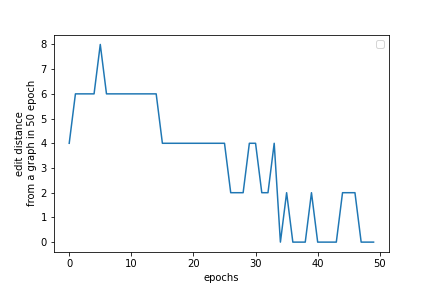
\includegraphics[clip,width=75mm]{graph.png}
		\caption{各学習時点のグラフと終了後のグラフとの編集距離}
		\label{fig:edit}
	\end{center}
\end{figure}

図\ref{fig:edit}に編集距離の変化を示した.
全体的な減少傾向から, グラフの収束に向かう様子が確認できた.
完全な収束判定は分からないが, 50 epoch付近でも変化があるためさらに学習時間を延ばして確認する必要がある.

\section{実験2}

探索したショートカット位置の性能を評価するため, アーキテクチャを探索する(a)探索段階, 探索したグラフ構造で学習する(b)評価段階, 素のVGGによる(c)ベースライン, の3つの精度を比較した.
設定は表\ref{tab:setting}を引き継ぐ.
実験は各1回, seed 41で行った.

\subsection{結果}

\begin{figure}[tb]
	\begin{center}
		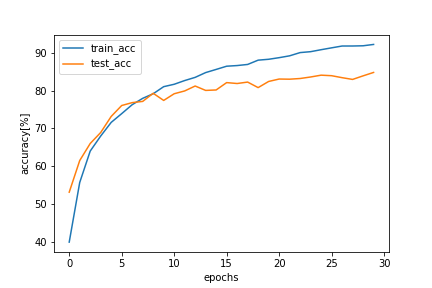
\includegraphics[clip,width=75mm]{search_acc.png}
		\caption{探索時のAccuracy}
		\label{fig:search_acc}
	\end{center}
\end{figure}

\begin{figure}[tb]
	\begin{center}
		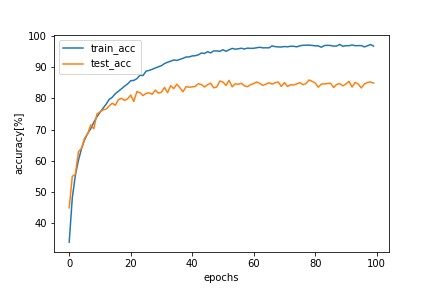
\includegraphics[clip,width=75mm]{eval_acc.png}
		\caption{評価時のAccuracy}
		\label{fig:eval_acc}
	\end{center}
\end{figure}

\begin{figure}[tb]
	\begin{center}
		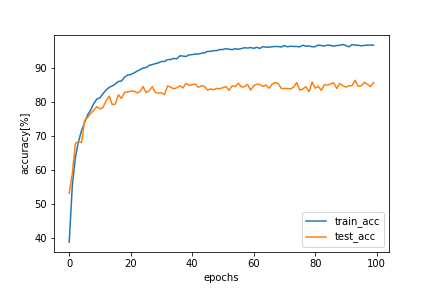
\includegraphics[clip,width=75mm]{baseline_acc.png}
		\caption{ベースライン(VGG11)のAccuracy}
		\label{fig:baseline_acc}
	\end{center}
\end{figure}

\begin{table}[tb]
  \begin{center}
    \caption{Accuracyの比較}
    \begin{tabular}{|c||c|c|} \hline
       & accuracy(\%) & 学習時間(epoch) \\ \hline \hline
      探索 & 84.78 & 30 \\ \hline
      評価 & 85.94 & 100 \\ \hline
      ベースライン & 86.26 & 100 \\ \hline
    \end{tabular}
    \label{tab:dist}
  \end{center}
\end{table}

図\ref{fig:search_acc}, \ref{fig:eval_acc}, \ref{fig:baseline_acc}に各訓練とテスト精度を,
表\ref{tab:dist}には最大テスト精度を示した.
評価時の精度は, 探索時より改善したものの, ベースラインよりも0.32 \%低くなった.

\subsection{考察}
今回の設定の場合, ショートカットを入れることで精度が低くなった.
原因として, ショートカット関数の問題と層の浅さが考えられる.

今回用いたショートカット関数は, 1x1 Conv(stride>=1)であり, 大きさの違う出力に対応するためstrideで無理やり補正している. strideが大きいほど, ショートカットによって情報が欠落することが精度に悪影響を与えていると思われる.
次回は情報が失われないショートカットに替える必要がある.

また層が浅いため, pooling層によって頻繁に大きさが変えられるため, ショートカットが行いにくく効果が薄い可能性がある. VGG19などより深いモデルの場合よりショートカットの効果が表れると推測される.

\section{今後の予定}
% なんとなくなんかの勉強をするとかではなく具体的に

\begin{itemize}
  \item ショートカット関数の改善
  \item VGG19への移植
\end{itemize}

\section{ソースコード}
% 埋め込みでもGitでもいいので参照できるように
githubのnotebookリポジトリ参照

% 参考文献リスト
\bibliographystyle{unsrt}
\bibliography{ref}
\end{document}
